\chapter{Media Item Ranking}
\label{cha:media-item-ranking}

% the code below specifies where the figures are stored
\ifpdf
    \graphicspath{{8_media_item_ranking/figures/PNG/}{8_media_item_ranking/figures/PDF/}{8_media_item_ranking/figures/}}
\else
    \graphicspath{{8_media_item_ranking/figures/EPS/}{8_media_item_ranking/figures/}}
\fi

\section{Introduction}

In the previous chapter, we have introduced methods
to deduplicate exact duplicate and near-duplicate media items.
In this chapter, we introduce ranking criteria and methods
to put deduplicated media clusters in a~well-defined order.
The application screenshots that can be seen in \autoref{fig:topvsfashionshow}
and \autoref{fig:topgrammy} show the
most intuitive ranking criterion one can imagine (besides publication time):
ranking by occurrence popularity.
The more often a~media item (or a~near-duplicate)
appears in any of the considered social networks, 
the higher it should be ranked.
However, ranking by occurrence popularity (or media item cluster size)
disregards one of the most valuable features of social networks: 
the social aspects.
In consequence, in this chapter, we will introduce
further media item ranking criteria that,
together with media item cluster size,
will allow us to come up with more adequate social media item ranking mechanisms.

\section{Evaluating Subjective Data}

Evaluating subjective data, like \emph{the} correct ranking
for a~set of media items, is a~challenging task.
For different users, there may be different optimal settings.
A~common subjective evaluation technique
is the \emph{Mean Opinion Score (MOS)}~\cite{itu1998mos}.
Traditionally, MOS is used for conducting subjective evaluations
of telephony network transmission quality,
however, more recently, MOS has also found
wider usage in the multimedia community
for evaluating inherently subjective things
like perceived quality from the users' perspective. 
Therefore, a~set of standard subjective tests are conducted,
where a~number of users rate the quality of test samples
with scores ranging from 1 (worst) to 5 (best).
The actual MOS is then the arithmetic mean of all individual scores.
Given a~subjective evaluation criterion
like the correctness of a~ranking,
MOS provides a~meaningful way to judge the overall quality of our approach.

\section{Media Item Ranking Criteria}

In this section, we describe several criteria that can serve to rank
media items retrieved from social networks. 
We base these criteria on the information available from
the media item extractors described in \autoref{cha:media-item-extraction},
which, given event-related search terms,
extract raw binary media items and associated microposts
from multiple social networks.

\paragraph{Textual Ranking Criteria:}

This category regards the microposts that accompany media items.
Typically, microposts provide a~description of media items.
Using named-entity disambiguation tools,
textual content can be linked to \emph{LOD} cloud concepts~\cite{steiner2011addingmeaning}.
We have described micropost annotation in detail in \autoref{cha:micropost-annotation}.

\paragraph{Visual Ranking Criteria:} \label{sec:visualrankingcriteria}

This category regards the contents of photos and videos.
We distinguish \emph{low-} and \emph{high-level} visual ranking criteria.
High-level criteria include logo detection,
face recognition, and camera shot separation.
Low-level criteria include file size, resolution,
duration of a~video, geolocation, and time.
Via \emph{Optical Character Recognition (OCR)}, contained characters can be treated as textual features.

\paragraph{Audial Ranking Criteria:}

This category regards the audio track of videos.
\emph{High-level} ranking criteria are the presence or absence
of silence, music, speech, or a~mixture thereof in videos.
Similar to visual features before,
audial \emph{low-level} features are the average bit rate,
volume, possibly distorted areas, \emph{etc.}
Through audio transcription, speech can be treated as textual features.

\paragraph{Social Ranking Criteria:}

This category regards social network effects like shares, mentions,
view counts, expressions of (dis)likes, user diversity, \emph{etc.}
Prior work~\cite{khrouf2012aggregatingsocialmedia}
allows us to not only examine these effects
on a~\emph{single} social network,
but in a~network-agnostic way across \emph{multiple} social networks.
We will detail social aspects more later on in this chapter.

\paragraph{Aesthetic Ranking Criteria:}

This category regards the desired outcome after the ranking, \emph{i.e.},
the media gallery that illustrates a~given event and its atmosphere.
Studies exist for the aesthetics of
automatic photo book layout~\cite{sandhaus2011photobook},
photo aesthetics \emph{per se}~\cite{obrador2012photoaesthetics},
video and music playlist generation~\cite{knees2006musicplaylist,davidson2010videorecommendation}.
However, to the best of our knowledge,
no media gallery composition aesthetics studies exist
that examine mixing video \emph{and} photo media items.

\paragraph{Temporal Ranking Criteria:}

This category regards the publication date of media items.
If media items are clustered, we use the youngest media item
as cluster representative.
Media items can be ranked by recency, as oftentimes more recent items
are more interesting in the streaming context of social networks.

\section{Social Interactions Abstraction Layer}
\label{sec:social-interactions-abstraction-layer}

As we have described in \autoref{cha:social-networks},
social networks have different paradigms of social interactions.
In \autoref{sec:data-format}, we have briefly presented the overall
abstraction layer on top of the native data formats
of all considered social networks in order to gain
a~network-agnostic view on the underlying social networks.
In this section, we detail the part of the abstraction layer
that models the network-specific social interaction patterns.
Those interaction patterns must be exposed by the social network 
via specific API calls in order to be considered,
which only is the case for a~subset of the social networks we deal with.
Social interaction data is to some extent the holy grail of social networks,
which is the reason why sometimes Web scraping is the last resort,
as outlined in more detail in \autoref{sec:media-item-extractors}.
In \autoref{table:social-interactions}, we have listed
how we abstract the social interactions in question on each social network.
In our concrete implementation, we differ unknown values
that are returned as \texttt{unknown}, \emph{i.e.},
where the information is not exposed,
from \texttt{0} values, where the value is known to be zero.
We briefly recall the social interactions part
of the abstraction layer's data format:

\begin{description}
  \item[\texttt{socialInteractions}] Container for social
    interactions
  \begin{description}  
  \item[\texttt{likes}] Number of times a~micropost was liked, or
    \texttt{unknown}
  \item[\texttt{shares}] Number of times a~micropost was shared, or
    \texttt{unknown}
  \item[\texttt{comments}] Number of comments a~micropost
    received, or \texttt{unknown}
  \item[\texttt{views}] Number of views a~micropost reached, or
    \texttt{unknown}
  \end{description}    
\end{description}

\begin{table}[!ht]
  \centering
  \small
  \begin{tabular}{|l|l|l|l|}
    \hline
    Likes & Shares & Comments & Views\\ \hline
    \pbox[t][4.5cm]{0.2\linewidth}{Facebook Like\\ \googleplus \plusone\\ Instagram Like\\ Flickr Favorite\\ YouTube Like\\ YouTube Favorite\\ Twitter Favorite} & \pbox[t][4.5cm]{0.2\linewidth}{Facebook Share\\ \googleplus Share\\ Twitter ReTweet} & \pbox[t][4.5cm]{0.4\linewidth}{Facebook Comments\\ \googleplus Comments\\ Instagram Comments\\ Twitter manual RT\\ Twitter @Replies\\ Twitpic Comments\\ MobyPicture Comments\\ Flickr Comments} & \pbox[t][4.5cm]{0.2\linewidth}{YouTube Views\\ Flickr Views\\ Twitpic Views\\ MobyPicture~Views}\\
      \hline
    \end{tabular}
    \caption[Abstract social network interaction paradigms]
      {Abstract social network interaction paradigms
      and their underlying native social network counterparts}
  \label{table:social-interactions}
\end{table}

\section{Merging and Ranking}
\label{sec:merging-social-interactions}

If a~set of media items is sufficiently similar to be clustered
under the criteria that were detailed in
\autoref{cha:media-item-deduplication},
we can treat the whole of the cluster
as if it were just one media item.
Therefore, we need to specify a~merging strategy
for the associated data of the individual media items
in the particular cluster.
\autoref{code:merging} shows the pseudocode of the merging algorithm.
During the merging step,
we treat unknown values represented as \texttt{unknown} as \texttt{0}.
The alternative to this solution would be to exclude \texttt{unknown} values
from the merging step.
However, as in practice a~considerable amount of
social interaction values are \texttt{unknwon},
we are forced to proceed with the abovementioned simplification.
The algorithm accumulates individual social interactions
and assigns the accumulated social interactions to the cluster.

\begin{lstlisting}[caption=The social interactions merging algorithm,
  label=code:merging, float=!ht, escapechar=§]
§\textbf{Input: cluster}§, cluster of visually similar media items 
§\textbf{Output: cluster}§, cluster with merged social interactions 

§\textbf{for}§ mediaItem §\textbf{in}§ cluster
  cluster.likes += isUnknown(mediaItem.likes) ? 0 : mediaItem.likes
  cluster.shares += isUnknown(mediaItem.shares) ? 0 : mediaItem.shares
  cluster.comments += isUnknown(mediaItem.comments) ? 0 : mediaItem.comments
  cluster.views += isUnknown(mediaItem.views) ? 0 : mediaItem.views
§\textbf{end for}§

§\textbf{return}§ cluster
\end{lstlisting}

\subsection{Selection of a~Cluster's Visual Representative}  

As outlined in the previous section, similar enough media items
are clustered and treated as just one media item.
The previous section introduced
a~merging algorithm for the social interactions data.
In this section, we introduce an algorithm for the selection of
a~cluster's visual representative.
Naturally, through the way the clustering algorithm works,
the contained media items are already visually similar. 
In consequence, we fall back to using \emph{low-level}
visual ranking criteria as defined in \autoref{sec:visualrankingcriteria}.
\autoref{code:clusterrepresentative} shows the cluster representative
selection algorithm, which is based on the low-level feature \emph{resolution}.
The algorithm selects the media item with the highest megapixel resolution
as the cluster representative.

\begin{lstlisting}[caption=Pseudocode of the cluster visual representative selection algorithm that finds the highest quality media item of a~cluster,
  label=code:clusterrepresentative, float, escapechar=§]
§\textbf{Input:}§ cluster, cluster of visually similar media items
§\textbf{Output:}§ cluster, cluster with visual representative
  
maxResolution = 0

§\textbf{for}§ mediaItem §\textbf{in}§ cluster
  
  §\textit{\# Ensure that videos will always be preferred}§  
  §\textbf{if}§ mediaItem.type == 'video' §\textbf{then}§
    mediaItem.width = mediaItem.height = INFINITY
  §\textbf{end if}§ 
    
  resolution = mediaItem.width * mediaItem.height
  §\textbf{if}§ resolution >= maxResolution §\textbf{then}§
    maxResolution = resolution
    cluster.representative = mediaItem
  §\textbf{end if}§  
§\textbf{end for}§

§\textbf{return}§ cluster     
\end{lstlisting}

\subsection{Ranking Formula}
\label{sec:introduction-of-a-ranking-formula}

Up to now, we have shown how media item clusters are formed,
how each cluster's social interactions data is accumulated,
and how a~cluster's representative media item is selected.
In this section, we describe a~ranking formula to rank
a~set of media clusters that match a~given query.
In the ranking formula, we consider several well-defined ranking criteria
that were detailed in~\cite{steiner2012definingaesthetic},
namely visual, audial, textual, temporal, social, and aesthetic.
For a~given set of media item clusters, a~ranking is calculated as follows.

\begin{gather}\label{eq:rankingformula}
  \alpha \times \mathit{likes} + \beta \times \mathit{shares} +
  \gamma \times \mathit{comments} + \delta \times \mathit{views} + \nonumber\\
  \epsilon \times \mathit{clusterSize} + \zeta \times \mathit{recency} +
  \eta \times \mathit{quality}
\end{gather}

The factors $ \mathit{likes}, \mathit{shares}, \mathit{comments},$ and $ \mathit{views} $
stem from the individual media items as described in \autoref{sec:social-interactions-abstraction-layer}
and \autoref{sec:merging-social-interactions}.
The factor $ \mathit{clusterSize} $ corresponds to the size of the current cluster. 
After some experimentation with different event media items sets,
the factor $ \mathit{recency} $ was empirically determined to be calculated as follows.
If the youngest media item in the cluster is less than or exactly one day old,
the value is 8, for two days it is 4, for three days it is 2,
and for each day more, the value is 1.
The factor $ \mathit{quality} $ is a~representation of the
presence of faces and a~media item's photo or video quality.
Empirically optimized default values
that can be fine-tuned for a~concrete media item set
were determined as follows:
$ \alpha = 2 $, $ \beta = 4 $ , $ \gamma = 8 $, $ \delta = 1 $,
$ \epsilon = 32 $, $ \zeta = 2 $, and $ \eta = 8 $.
These factors follow the usage patterns of the different actions:
viewing happens more often than liking, which in turn happens more often than commenting.
We describe the evaluation in the upcoming section.

\section{Evaluation Based on the Super Bowl XLVII Event}
\label{sec-chapter7-evaluation}

\subsection{Super Bowl Analyses by Social Networks}

We have evaluated our approach with the (at time of writing)
recent event of the Super Bowl XLVII%
\footnote{\url{http://en.wikipedia.org/wiki/Super_Bowl_XLVII},
accessed February 8, 2013}.
This event received broad social media coverage, and the social networks
Twitter\footnote{\url{http://blog.twitter.com/2013/02/the-super-tweets-of-sb47.html},
accessed February 8, 2013},
Instagram\footnote{\url{http://blog.instagram.com/post/42254883677/sbroundup},
accessed February 8, 2013}, and
Facebook\footnote{\url{http://newsroom.fb.com/News/570/Super-Bowl-XLVII-on-Facebook},
accessed February 8, 2013} all published blog posts with analyses of the event
on the respective networks,
whereas the search engine Google%
\footnote{\url{http://googleblog.blogspot.com/2013/02/m-beyonce-and-ravens-dominate-game-day.html},
accessed February 8, 2013}
published an analysis of trending queries during the match.
In the following, we provide summaries of these different analyses,
with the expectation to encounter relevant media items
for each of the mentioned highlights in the final ranked list of media items
stemming from the various social networks.

According to Twitter's analysis,%
\footnote{\url{http://blog.twitter.com/2013/02/the-super-tweets-of-sb47.html},
accessed February 8, 2013}
the five moments that generated the most tweets
during the game (see the Wikipedia-provided game summary
\footnote{\url{http://en.wikipedia.org/wiki/Super_Bowl_XLVII},
accessed February 8, 2013} for details)
ordered by decreasing number of tweets per minute were
the power outage,
the 108-yard kickoff return for the Ravens touchdown by Jones,
the moment when the clock expired and the Ravens won,
Jones catches a~56 yard pass for a~Ravens touchdown,
and the Gore touchdown for the 49ers.
Overall, 24.1 million tweets about the game and halftime show were counted,
a~number that even leaves aside the advertisements.
The Twitter article further mentions the performance by superstar artist Beyoncé 
and a~number of Super Bowl advertisements as highlights of the event.   

Instagram's analysis\footnote{\url{http://blog.instagram.com/post/42254883677/sbroundup},
accessed February 8, 2013}
mentions that more than three million photos
with Super Bowl-related words in their captions were shared and
at peak more than 450 photos about the game were posted every second.
During the halftime show, over 200 photos per second were posted about Beyoncé.
The blog post further highlights how a~TV channel pointed to selected photos
and explains that brands ran Instagram campaigns.
According to Instagram, people used Instagram both directly at the event venue,
but also while watching from home, either by photographing their TV sets,
or by photographing each other how they watched the event.

Facebook's analysis\footnote{\url{http://newsroom.fb.com/News/570/Super-Bowl-XLVII-on-Facebook},
accessed February 8, 2013}
mentions as top five most-talked-about moments of the Super Bowl 
the moment when the Ravens win the Super Bowl, 
Beyoncé's halftime performance,
the power outage in the Superdome,
Jacoby Jones' 108-yard kickoff return for a~Ravens touchdown, and
Joe Flacco’s 56-yard pass to Jacoby Jones for a~Ravens touchdown.
The Super Bowl was nicknamed the Harbaugh Bowl, as both teams' head coaches
are named Harbaugh as last name.
Facebook also mentions Alicia Keys' performance of the National Anthem as special event.

The search engine Google has compiled a~list of top trending search terms
during the match, with the top ones being the sponsor M\&M's, Beyoncé, Baltimore Ravens,
San Francisco 49ers, and Colin Kaepernick (quarterback for the San Francisco 49ers).
Additional spiking search terms were power outage
and Chrysler (driven by an advertisement during the game).
Further advertisement-related search terms were for advertisements for M\&M's,
Mercedes-Benz, Disney’s Oz Great and Powerful movie, Lincoln, and Audi.

While no separate statistics are available yet at time of writing
for the video hosting platform YouTube,
Google's blog post mentions that searches for Gangnam Style were trending on YouTube,
along with searches for big game performers Alicia Keys and Beyoncé.

\subsection{Expected Super Bowl Media Items}

Given the previous social network analyses, we expect to see media items
on the following topics (in no particular order):

\begin{itemize}
  \itemsep0em
  \item the power outage
  \item the performances of Beyoncé and Alicia Keys
  \item the advertisements
  \item the match itself from people at the stadium
  \item the Super Bowl watchers around the world 
\end{itemize}

\autoref{fig:loose_order} and \autoref{fig:strict_order} show media items
for the two queries 49ers and Baltimore Ravens arranged
in two different media gallery styles, loose order and strict order.
For details on media gallery generation, we refer the reader to the upcoming
\autoref{cha:media-item-compilation}.

\begin{figure}[!ht]
  \centering
  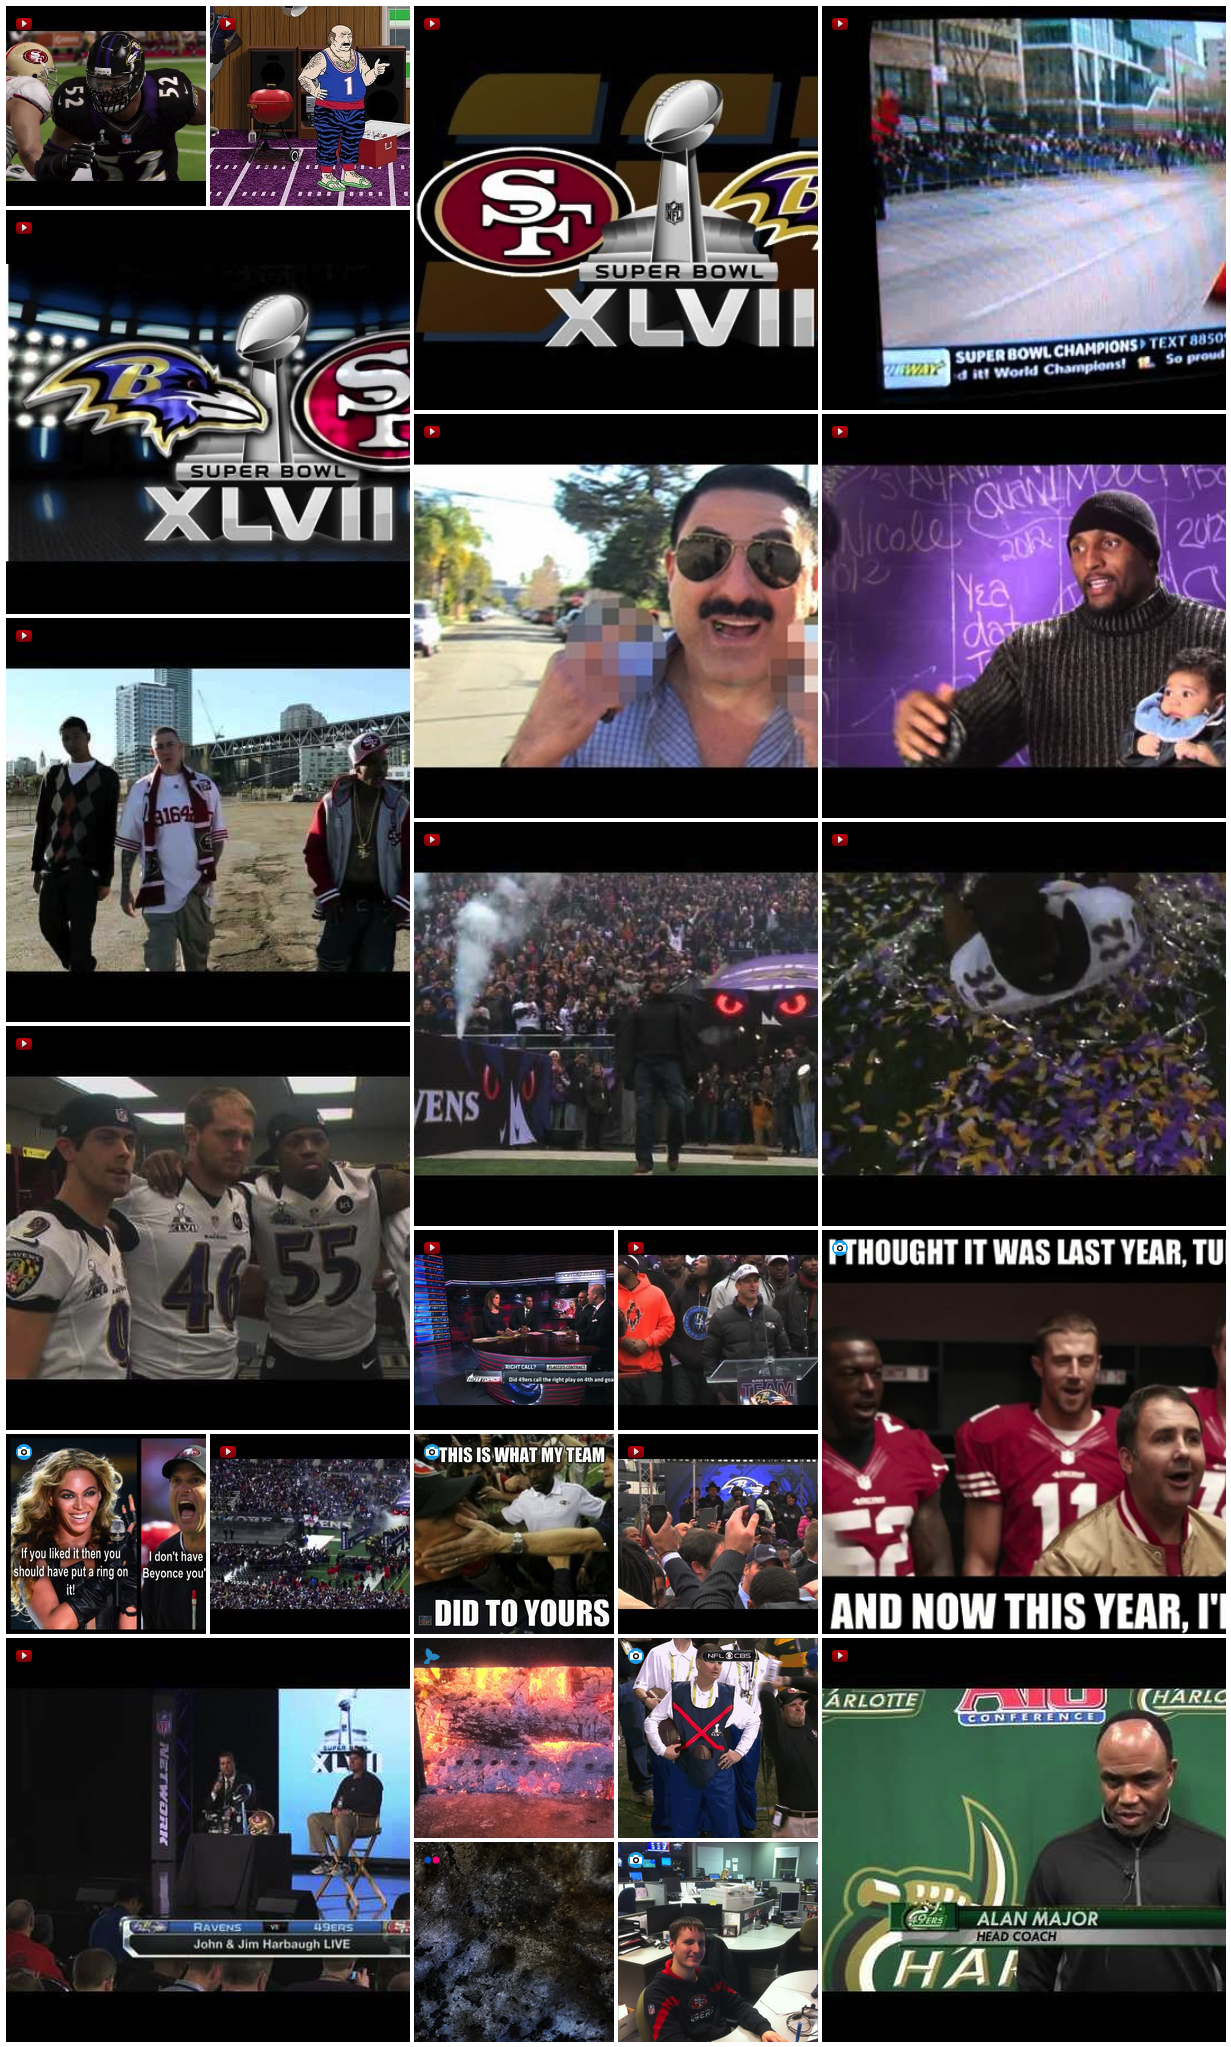
\includegraphics[width=0.95\textwidth,height=0.9\textheight,keepaspectratio]{loose_order.png}
  \caption[Ranked Super Bowl media gallery in loose order]
  {Ranked Super Bowl media gallery in loose order}
  \label{fig:loose_order}
\end{figure}

\begin{sidewaysfigure}
  \centering
  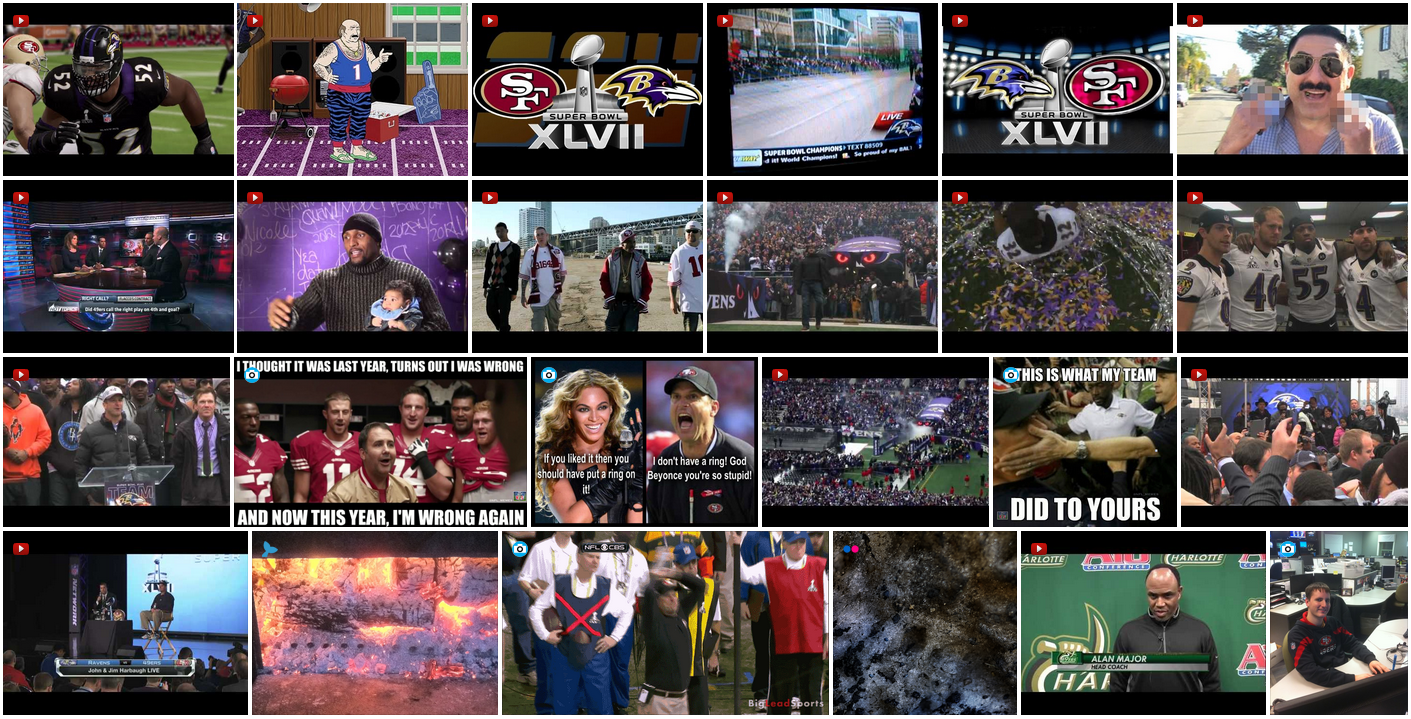
\includegraphics[width=0.95\textwidth,height=0.9\textheight,keepaspectratio]{strict_order.png}
  \caption[Ranked Super Bowl media gallery in strict order]
  {Ranked Super Bowl media gallery in strict order \todo{Check final orientation}}
  \label{fig:strict_order}
\end{sidewaysfigure}  

\subsection{Evaluation Approach}

We asked three human raters to agree on a~rating for the media items
that were retrieved for the two queries 49ers and Baltimore Ravens.
We have made the dataset of media items available%
\footnote{\url{https://www.dropbox.com/sh/30qwuvphcv49max/ilsaMbSdf6},
accessed February 12, 2013}.
We then fine-tuned the weight factors
$ \alpha, \beta, \gamma, \delta, \epsilon, \zeta $, and $ \eta $ of the ranking formula
that was introduced in \autoref{sec:introduction-of-a-ranking-formula}
until the highest possible agreement between the human-generated ranking
and the system-generated ranking was reached.
Afterwards, we tested these empirically determined weight factors of the ranking formula
with different events and asked the evaluators to what extent
on a~MOS scale from 1--5 they agreed with each of the top-10 ranked media items.
Rating the ranking of all media items is barely possible,
which is why we limit ourselves to rating the top-10 returned results,
a~technique that is also known as \emph{pooling}
in the Information Retrieval community~\cite{liu2009learningtorank}.
Screenshots of some of the events we tested with
and the particular top-ranked media items can be seen in 
\autoref{fig:qualcomm}, \autoref{fig:blackberry}, and \autoref{fig:facebookgraphsearch}.

\begin{figure}[!ht]
  \centering
  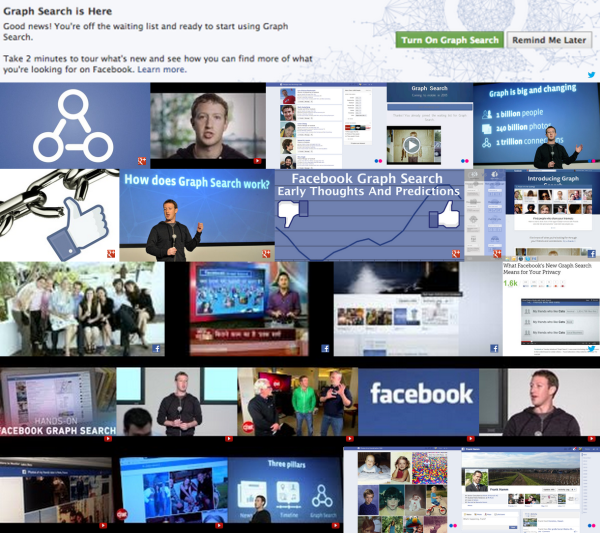
\includegraphics[width=0.75\linewidth]{facebook.png}
  \caption[Ranked media gallery for the Facebook Graph Search launch event]
  {Ranked media gallery for the Facebook Graph Search launch event
  on January 15, 2013}
  \label{fig:facebookgraphsearch}
\end{figure}

\begin{figure}[!ht]
  \centering
  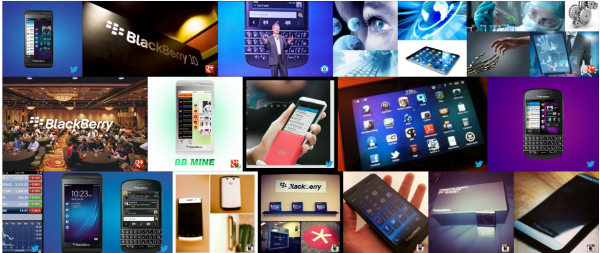
\includegraphics[width=0.75\linewidth]{blackberry.png}
  \caption[Ranked media gallery for the BlackBerry 10 launch event]
  {Ranked media gallery for the BlackBerry 10 launch event on January 30, 2013}
  \label{fig:blackberry}
\end{figure}

\begin{figure}[!ht]
  \centering
  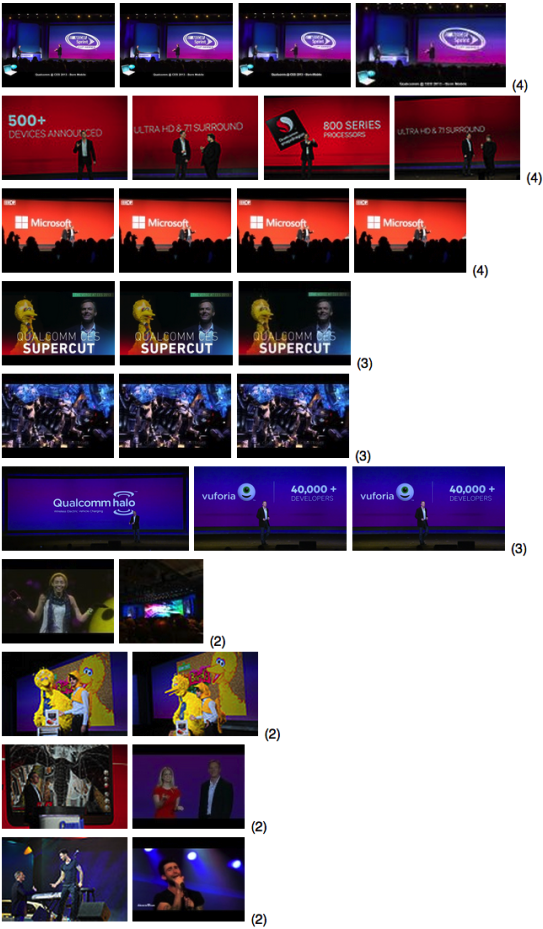
\includegraphics[width=0.95\textwidth,height=0.9\textheight,keepaspectratio]{qualcomm.png}
  \caption[Ranked media items for the Qualcomm CES 2013 keynote event]
  {Ranked media items for the Qualcomm CES 2013 keynote event
  on January~8, 2013 (raw cluster view)}
  \label{fig:qualcomm}
\end{figure}

\subsection{Evaluation Results}

In this subsection, we present the human rater results
in the form of MOS scores of the events
that we tested our ranking formula with.
As can be seen in \autoref{table:top-10-mos}
and as the combined MOS of 3.7 (variance 0.8) suggests,
all selected top-10 media items
were overall considered relevant by the human raters.
We arranged for post-test conversations with each human rater
in order to understand their motivations for their ratings.
After talking to the human raters it became clear that
lower scores were mostly caused by outliers in the media item set.
Post-test conversations with the human raters revealed that 
if at a~first glance the context to the event in question was missing,
this fact made them heavily downgrade the corresponding media items.
We note that in order to test the visual ranking aspect in isolation,
raters were exclusively shown media items
without any micropost context.
This approach made it hard for them to recognize connections
between \emph{remote} media items to events \emph{on-site}.
Examples of remote media items are media items of Super Bowl watchers
around the world or photo montages of online news media
(Facebook Graph Search launch, BlackBerry~10 launch).
Another reason for outliers according to the raters
were too small media item previews of
videos that only made sense when seen in motion.

\begin{table}
  \centering
  \small
  \begin{tabular}{|l|l|l|l|l|l|l|l|l|l|l|l|l|}
    \hline
    \backslashbox{\textbf{Event}}{\textbf{Rank}} & \textbf{1} & \textbf{2} & \textbf{3} & \textbf{4} & \textbf{5} & \textbf{6} & \textbf{7} & \textbf{8} & \textbf{9} & \textbf{10} & \textbf{avg} & \textbf{var} \\ \hline
    \textbf{Facebook} & 3.8 & 3.3 & 4.9 & 4.2 & 3.9 & 5.0 & 3.7 & 4.8 & 4.8 & 3.1 & \textbf{3.6} & \textbf{0.4}\\ \hline
    \textbf{BlackBerry} & 4.9 & 4.8 & 5.0 & 3.2 & 5.0 & 4.4 & 4.1 & 3.8 & 4.5 & 2.7 & \textbf{3.8} & \textbf{0.8} \\ \hline
    \textbf{Qualcomm}& 4.9 & 4.7 & 4.9 & 5.0 & 2.4 & 4.1 & 3.1 & 5.0 & 2.1 & 3.7 & \textbf{3.6} & \textbf{1.0} \\ \hline 
    \textbf{Super Bowl}& 5.0 & 4.1 & 5.0 & 3.2 & 5.0 & 2.8 & 4.1 & 4.6 & 3.3 & 4.0 & \textbf{3.9} & \textbf{0.9} \\
    \hline
  \end{tabular}
  \caption[Mean Opinion Scores (MOS) for top-10 ranked media items]
    {Mean Opinion Scores (MOS) for the top-10 ranked media items of four events (overall MOS: 3.7, variance: 0.8)}
  \label{table:top-10-mos} 
\end{table}

\section{Conclusion}

In this chapter, we have discussed MOS as a~method
for evaluating subjective data.
In continuation, we have detailed criteria
that can be considered for the creation of a~ranking.
We have shown how we abstract social interactions on social networks
and introduced an algorithm to merge social interactions
when media items are clustered.
Additionally, we have further detailed an algorithm
for the selection of a~media item cluster's visual representative.
Finally, we have used the previously introduced pieces
for the definition of a~ranking formula,
whose weight factors we have empirically determined with one event
and successfully evaluated in practice with three other events.

For the task of ranking media items, there is no one correct solution,
but only optimizations under given constraints.
Albeit a~maximum agreement between human raters is aimed for,
individual users will always have different ranking needs.
With our ranking formula proposition, we want to help
such individual users with a~rationally traceable and useful default ranking
that can be adapted easily to special needs, or media item sets.
We have implemented this ranking formula in a~stand-alone application,%
which will be described in more detail in \autoref{sec:socialmediaillustrator}.
Within this application,
users can easily modify the weight factors
to see their effects on-the fly.
Besides all possible customization,
the application still proposes reasonable default values
for each individual parameter that have been demonstrated
to work well for the majority of cases.
\autoref{fig:social-media-illustrator} shows a~screenshot of this application
that effectively helps users see the media items needles first, and the haystack last.

\begin{figure}[!ht]
  \centering
  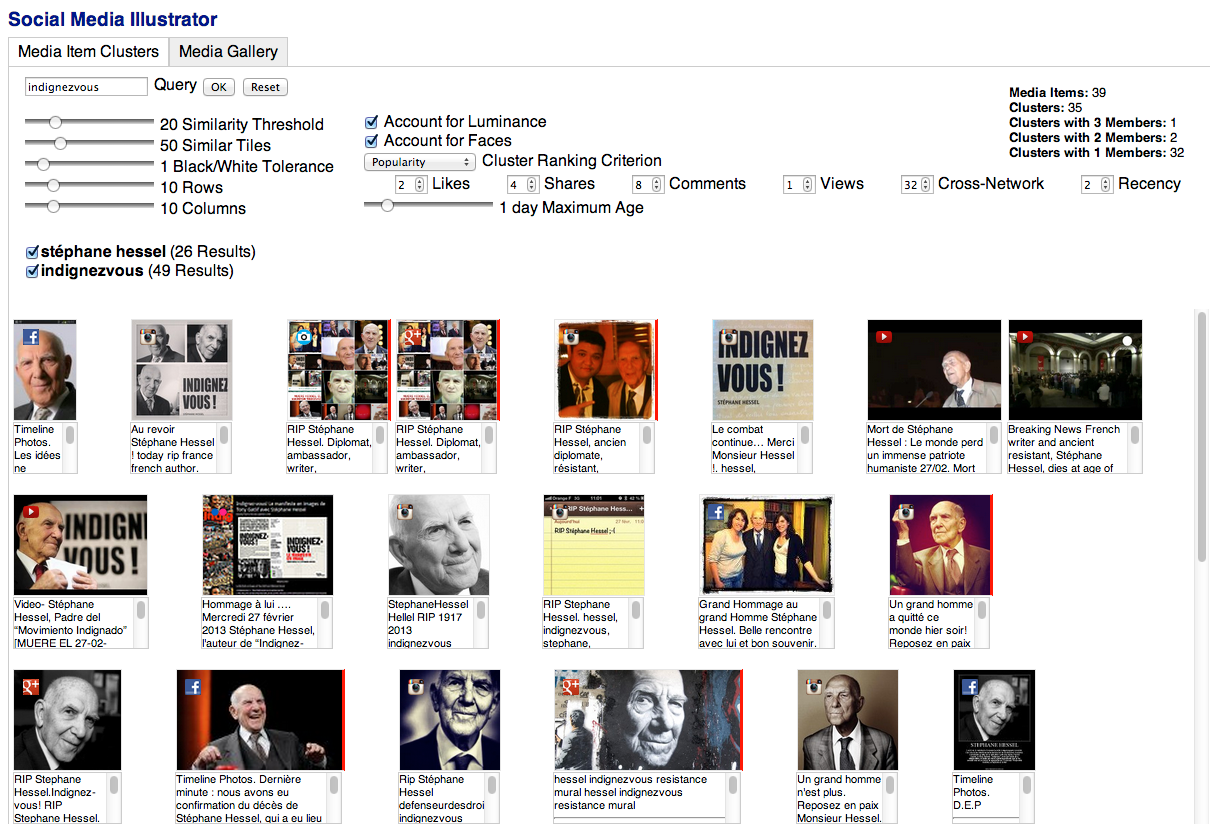
\includegraphics[width=1.0\linewidth]{social-media-illustrator.png}
  \caption[Media item ranking in our application with adjustable weight factors]
  {Media item ranking in our application with adjustable weight factors for the ranking formula}
  \label{fig:social-media-illustrator}
\end{figure}


\section*{Chapter Notes}
This chapter is partly based on the following publications:
\todo{Add publications}

\bibliographystyle{plainnat}
\bibliography{backmatter/references}
